% Chương 1 - Nguồn: TV2 (Đình Bảo), Google Doc "Workspace Nhóm - BTL Vật Lý 1 2026"
\chapter{CƠ SỞ LÝ THUYẾT VẬT LÝ VỀ CHUYỂN ĐỘNG NÉM XIÊN}\label{chap:lythuyet}

\section{Các giả thiết lý tưởng và thiết lập hệ trục tọa độ Oxy}

\subsection{Định nghĩa}
Ném xiên là chuyển động của một vật được ném lên với một vận tốc ban đầu hợp với phương ngang một góc $\alpha$ và vật chỉ chịu tác dụng của trọng lực.

\subsection{Các giả thiết}
\begin{itemize}
  \item Bỏ qua mọi lực cản của không khí tác dụng lên vật.
  \item Xem vật là chất điểm.
  \item Gia tốc trọng trường $\vec{g}$ là hằng số, không đổi cả về hướng lẫn độ lớn, do độ cao bay và tầm xa rất nhỏ so với bán kính Trái Đất.
  \item Mặt đất được coi là mặt phẳng ngang; hệ quy chiếu gắn với mặt đất được coi là hệ quy chiếu quán tính (bỏ qua sự tự quay của Trái Đất, do đó bỏ qua lực quán tính Coriolis).
\end{itemize}

\subsection{Ký hiệu và đơn vị}
Các đại lượng đã cho:
\begin{itemize}
  \item Vận tốc ban đầu $v_0$: tốc độ tại thời điểm vật bắt đầu được ném, $v_0 > 0$ (m/s).
  \item Góc ném $\alpha$: góc hợp bởi vectơ vận tốc ban đầu và phương ngang Ox, với $0^\circ < \alpha < 90^\circ$ (đơn vị: độ hoặc rad).
  \item Gia tốc trọng trường $g$: gia tốc do lực hút Trái Đất gây ra, luôn hướng thẳng đứng xuống dưới (lấy bằng $9{,}81~\mathrm{m/s^2}$).
\end{itemize}
Các đại lượng cần xác định:
\begin{itemize}
  \item $R$: tầm ném xa (m).
  \item $H$: độ cao cực đại (m).
  \item $T$: thời gian bay (s).
\end{itemize}

\subsection{Hệ tọa độ Oxy}
\begin{itemize}
  \item Gốc tọa độ O: đặt tại vị trí ném vật ở thời điểm ban đầu $t = 0$.
  \item Trục Ox: nằm ngang, hướng theo chiều hình chiếu ngang của vận tốc ban đầu.
  \item Trục Oy: thẳng đứng, hướng lên trên (xem Hình~\ref{fig:nemxien}).
\end{itemize}

\begin{figure}[H]
  \centering
  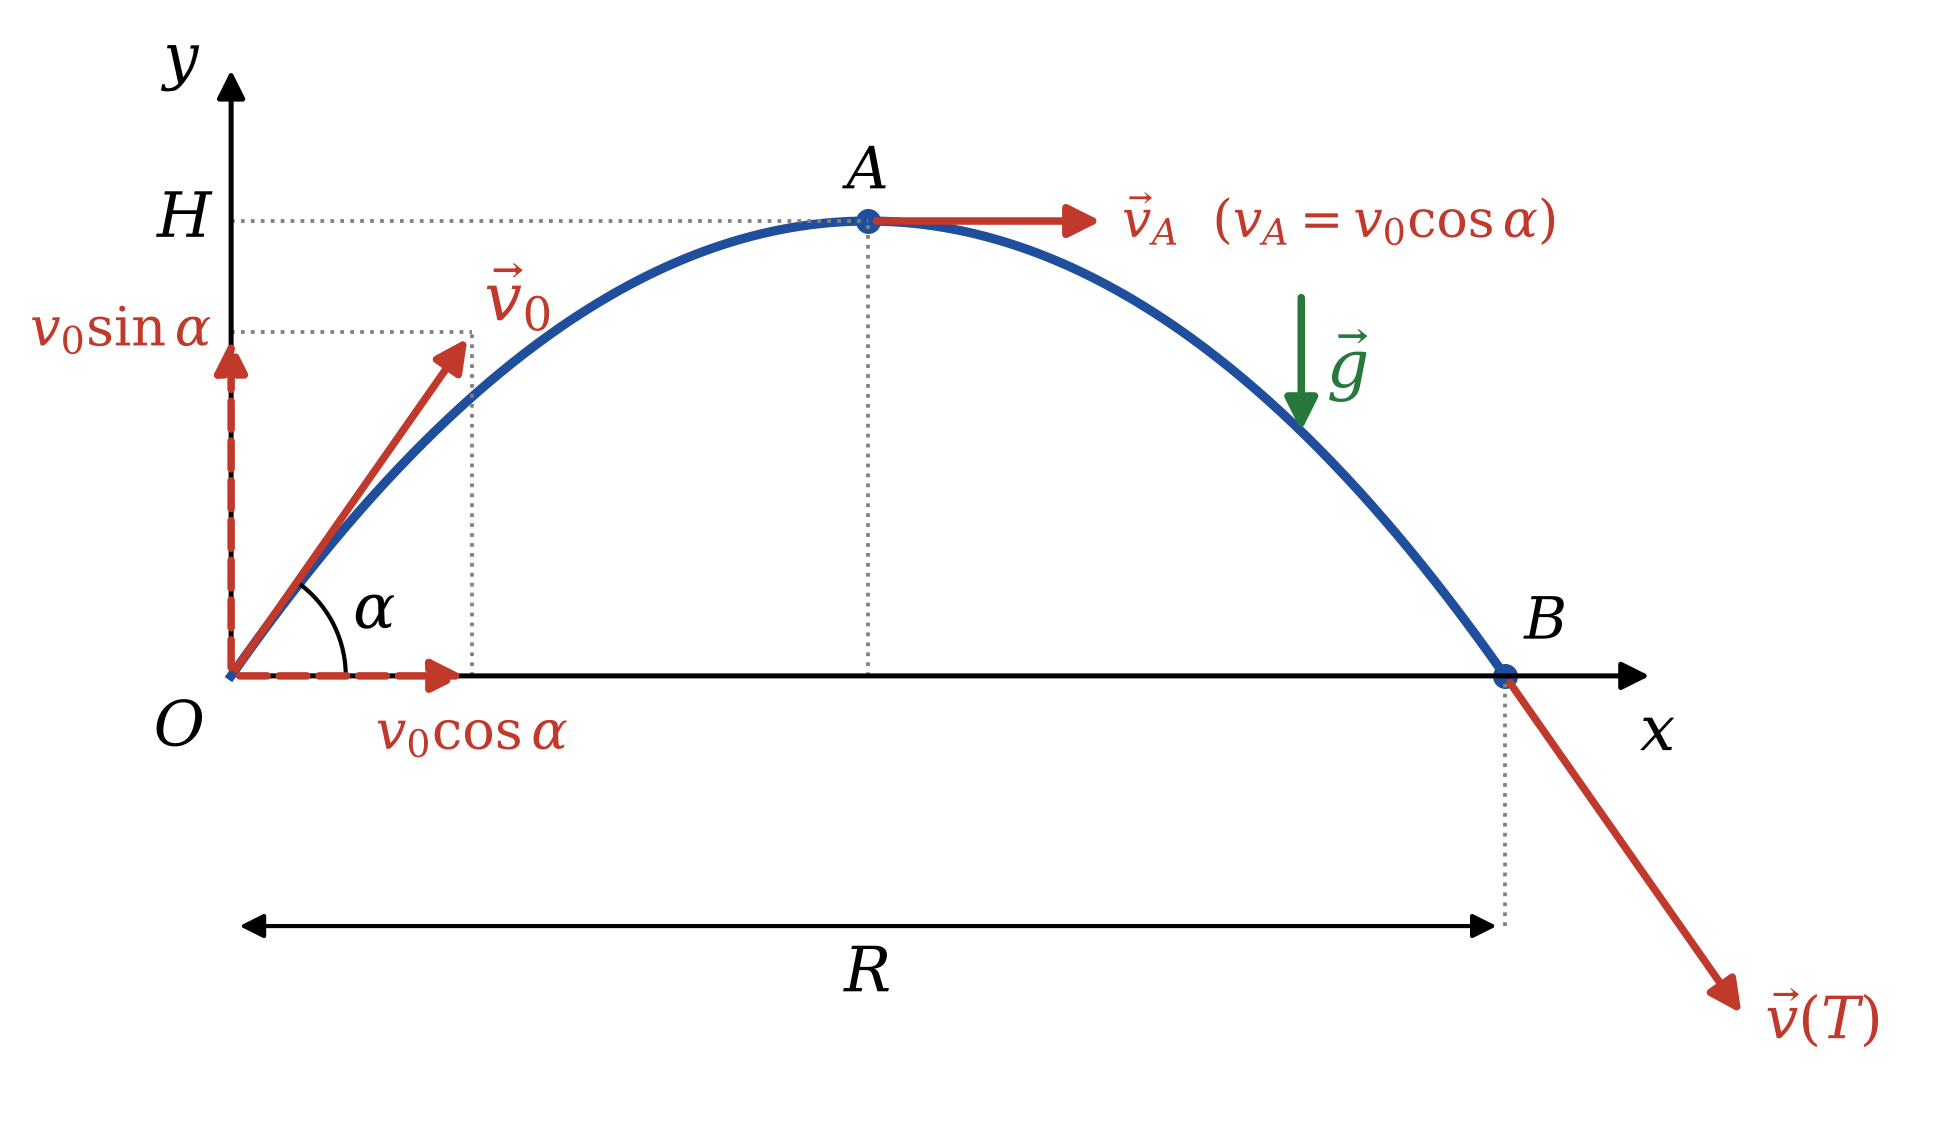
\includegraphics[width=0.85\textwidth]{hinh1_1_nemxien.png}
  \caption{Quỹ đạo chuyển động ném xiên và các đại lượng đặc trưng trong hệ tọa độ Oxy}
  \label{fig:nemxien}
\end{figure}

\section{Phương trình vi phân chuyển động và quy luật động học}
Theo định luật II Newton, phương trình vectơ chuyển động của vật chỉ chịu tác dụng của trọng lực $\vec{P} = m\vec{g}$ là:
\[ m\vec{a} = \vec{P} = m\vec{g} \]
Suy ra:
\[ \vec{a} = \vec{g} \]
Như vậy, gia tốc của vật bằng gia tốc trọng trường $\vec{g}$ và không phụ thuộc vào khối lượng $m$ của vật. Chiếu phương trình vectơ này lên hai trục tọa độ, ta thu được các phương trình sau.

Phương trình vi phân:
\begin{itemize}
  \item Trục Ox: $a_x = \dfrac{\mathrm{d}^2x}{\mathrm{d}t^2} = 0$: chuyển động hình chiếu trên trục Ox là chuyển động thẳng đều.
  \item Trục Oy: $a_y = \dfrac{\mathrm{d}^2y}{\mathrm{d}t^2} = -g$: chuyển động hình chiếu trên trục Oy là chuyển động thẳng biến đổi đều. Dấu ``$-$'' xuất hiện vì $\vec{g}$ ngược chiều trục Oy ($g > 0$ là độ lớn gia tốc trọng trường).
\end{itemize}

Tại thời điểm ban đầu $t = 0$, vật được ném từ gốc tọa độ với vận tốc ban đầu $v_0$ hợp với phương ngang góc $\alpha$:
\begin{itemize}
  \item Tọa độ ban đầu: $x(0) = 0$, \ $y(0) = 0$.
  \item Vận tốc ban đầu: $v_x(0) = v_0\cos\alpha$, \ $v_y(0) = v_0\sin\alpha$.
\end{itemize}

Vận tốc theo thời gian: lấy tích phân hai vế phương trình vi phân gia tốc theo thời gian $t$, sau đó thay vận tốc ban đầu, ta được phương trình vận tốc:
\begin{align*}
  v_x(t) &= \int 0\,\mathrm{d}t = C_1,
    & \text{tại } t = 0:\ v_x(0) &= v_0\cos\alpha \;\Rightarrow\; C_1 = v_0\cos\alpha \\
  v_y(t) &= \int (-g)\,\mathrm{d}t = -gt + C_2,
    & \text{tại } t = 0:\ v_y(0) &= v_0\sin\alpha \;\Rightarrow\; C_2 = v_0\sin\alpha
\end{align*}
Suy ra:
\[ v_x(t) = v_0\cos\alpha, \qquad v_y(t) = -gt + v_0\sin\alpha \]

Phương trình tọa độ: tiếp tục lấy tích phân hai vế phương trình vận tốc theo thời gian $t$, sau đó áp dụng điều kiện tọa độ ban đầu, ta được:
\[ x(t) = \int v_0\cos\alpha\,\mathrm{d}t = (v_0\cos\alpha)\,t + C_3; \qquad x(0) = 0 \Rightarrow C_3 = 0 \]
\begin{equation}
  x(t) = v_0\cos\alpha\cdot t
  \label{eq:x}
\end{equation}
\[ y(t) = \int (-gt + v_0\sin\alpha)\,\mathrm{d}t = -\frac{1}{2}gt^2 + (v_0\sin\alpha)\,t + C_4; \qquad y(0) = 0 \Rightarrow C_4 = 0 \]
\begin{equation}
  y(t) = -\frac{1}{2}gt^2 + v_0\sin\alpha\cdot t
  \label{eq:y}
\end{equation}

\section{Phương trình quỹ đạo chuyển động}
Để xác định phương trình quỹ đạo, trước tiên ta rút $t$ theo $x$ từ phương trình \eqref{eq:x}:
\[ t = \frac{x}{v_0\cos\alpha} \]
Thay biểu thức $t$ theo $x$ vào phương trình \eqref{eq:y}, ta được:
\[ y = \frac{v_0\sin\alpha\cdot x}{v_0\cos\alpha} - \frac{1}{2}g\left(\frac{x}{v_0\cos\alpha}\right)^2 \]
Rút gọn biểu thức trên, ta có:
\begin{equation}
  y = x\tan\alpha - \frac{g\,x^2}{2v_0^2\cos^2\alpha}
  \label{eq:quydao}
\end{equation}
Đây là phương trình bậc hai có dạng $y = ax^2 + bx + c$, trong đó:
\begin{itemize}
  \item $b = \tan\alpha$, \ $c = 0$;
  \item $a = -\dfrac{g}{2v_0^2\cos^2\alpha} < 0$.
\end{itemize}
Vì hệ số $a$ âm nên đạo hàm bậc hai của hàm số luôn âm. Do đó, quỹ đạo của chuyển động ném xiên là một đường parabol có bề lõm hướng xuống dưới. Phương trình \eqref{eq:quydao} chỉ áp dụng khi $\alpha \neq 90^\circ$ (vì khi rút $t$ theo $x$ đã chia cho $\cos\alpha$) và chỉ có nghĩa trong đoạn $0 \le x \le R$.

\section{Thiết lập công thức giải tích cho tầm xa \texorpdfstring{($R$)}{(R)}, độ cao cực đại \texorpdfstring{($H$)}{(H)} và thời gian bay \texorpdfstring{($T$)}{(T)}}
Các công thức dưới đây áp dụng khi vật được ném từ mặt đất và rơi trở lại cùng độ cao ban đầu.

\subsection{Thời gian bay \texorpdfstring{($T$)}{(T)}}
Vật chạm đất khi tọa độ theo phương thẳng đứng trở về giá trị ban đầu, tức là $y = 0$.

Thay $y = 0$ vào phương trình \eqref{eq:y}, sau đó phân tích thành nhân tử. Bỏ nghiệm $t = 0$ tương ứng với thời điểm bắt đầu ném, nghiệm còn lại là thời gian bay $T$:
\[ t\left(v_0\sin\alpha - \frac{gt}{2}\right) = 0 \;\Rightarrow\; t = 0 \ \text{hoặc}\ t = T \]
\begin{equation}
  T = \frac{2v_0\sin\alpha}{g}
  \label{eq:T}
\end{equation}

\subsection{Độ cao cực đại \texorpdfstring{($H$)}{(H)}}
Tại điểm cao nhất A của quỹ đạo (Hình~\ref{fig:nemxien}), vận tốc theo phương thẳng đứng bằng 0, tức là $v_y = 0$.

Từ phương trình vận tốc theo thời gian, suy ra thời điểm vật đạt độ cao cực đại:
\[ t_H = \frac{v_0\sin\alpha}{g} \]
So sánh với \eqref{eq:T}, ta có:
\[ t_H = \frac{T}{2} \]
Điều này cho thấy thời gian vật đi lên bằng thời gian vật đi xuống khi vật được ném và rơi trở lại cùng một độ cao.

Để xác định độ cao cực đại, thay $t_H = v_0\sin\alpha/g$ vào phương trình \eqref{eq:y}, quy đồng mẫu số và rút gọn, ta thu được công thức cuối cùng:
\begin{equation}
  H = v_0\sin\alpha\cdot t_H - \frac{g\,t_H^2}{2}
    = \frac{v_0^2\sin^2\alpha}{g} - \frac{v_0^2\sin^2\alpha}{2g}
    = \frac{v_0^2\sin^2\alpha}{2g}
  \label{eq:H}
\end{equation}

\subsection{Tầm xa \texorpdfstring{($R$)}{(R)}}
Tầm xa là khoảng cách theo phương ngang từ điểm ném O đến điểm rơi B của vật (Hình~\ref{fig:nemxien}). Khi vật chạm đất, $t = T$.

Thay $T = 2v_0\sin\alpha/g$ vào phương trình \eqref{eq:x}, rút gọn và sử dụng công thức lượng giác:
\[ \sin 2\alpha = 2\sin\alpha\cos\alpha \]
Suy ra công thức tính tầm xa:
\begin{equation}
  R = v_0\cos\alpha\cdot T = \frac{2v_0^2\sin\alpha\cos\alpha}{g} = \frac{v_0^2\sin 2\alpha}{g}
  \label{eq:R}
\end{equation}
Kiểm tra thứ nguyên: $[v_0^2/g] = (\mathrm{m^2/s^2})/(\mathrm{m/s^2}) = \mathrm{m}$, nên $R$ và $H$ có đơn vị mét; $[v_0/g] = (\mathrm{m/s})/(\mathrm{m/s^2}) = \mathrm{s}$, nên $T$ có đơn vị giây.

\subsection{Vận tốc lúc chạm đất}
Tại thời điểm chạm đất $t = T$:
\[ v_x(T) = v_0\cos\alpha; \qquad v_y(T) = v_0\sin\alpha - gT = -v_0\sin\alpha \]
Do đó độ lớn vận tốc lúc chạm đất bằng $v_0$; vectơ vận tốc hướng xuống và hợp với phương ngang góc $\alpha$. Kết quả này phù hợp với định luật bảo toàn cơ năng vì điểm ném và điểm rơi ở cùng độ cao.
